\documentclass[12pt]{article}
\usepackage{graphicx}
\usepackage{booktabs}
\usepackage[margin=1.0in]{geometry}
\usepackage{color}
\usepackage{tabularx}
%Times New Roman 12 pt
\usepackage[T1]{fontenc}
\usepackage{mathptmx}
\usepackage{amssymb}
\usepackage{amsmath}
\usepackage{authblk}
\usepackage[backend=bibtex,style=phys]{biblatex}

\graphicspath{{snapshots/}}

\newcommand{\angstrom}{\textup{\AA}}

\title{}
\author[1]{Lisa E. Felberg}
\author[2]{Luis A. Ruiz Pestana} 
\author[1-4]{Teresa Head-Gordon} 

\addbibresource{references}

\affil[1]{Department of Chemical and Biomolecular Engineering, University of California Berkeley, 
Berkeley, California 94720, USA}
\affil[2]{Chemical Sciences Division, Lawrence Berkeley National Labs
Berkeley, California 94720, USA}
\affil[3]{Department of Chemistry, University of California Berkeley, 
Berkeley, California 94720, USA}
\affil[4]{Department of Bioengineering, University of California Berkeley, 
Berkeley, California 94720, USA}


\date{}
\setcounter{Maxaffil}{0}
\renewcommand\Affilfont{\itshape\small}

\begin{document}
	\maketitle
\clearpage

\section*{Abstract}

\clearpage

\section*{Introduction}

Significance: many simulations have been performed with rigid graphene models, but if they are flexible, they may interact with the water in in different ways.

Previous studies on confined water:

1. Water in rigid graphene

2. Water in flexible graphene - used finite graphene sheets, did not observe 

\clearpage

\section*{Methods}

\subsection*{Models}

For this study, simulations of systems with parallel graphene plates with
separations of 6 and 12 \r A respectively in the x-cartesian dimension.
Systems of two different sizes were used to explore periodic size effects, with graphene
plate separation held constant. The smaller systems had y-z dimensions of 46.2 by 48.5 \r A
and the large systems had dimensions of 121.8 by 118.8 \r A.

\textbf{\color{red} How were they built?? }

\subsection*{Force fields}

Harmonic bond and angle potentials were applied to the graphene sheets with 
the following parameters: k\textsubscript{bond} = 938.0 \(kCal/mol/\angstrom^2\)
and k\textsubscript{angle} = 126.0 \(kCal/mol/rad^2\), equilibrium bond and 
angle lengths of 1.40 \r A and 120.0 degrees respectively \cite{Hummer2001}. The
dihedral potential is harmonic with the functional form: \(E_{\text{di}} = K_{\text{di}} [ 1 + d cos(\phi)]\),
where K\textsubscript{di} = 3.15 kCal/mol, \(\phi = 180.0\) degrees and \(d = \pm 1\) \cite{Patra2009}. An improper torsional 
potential with a harmonic functional form as follows: \( E_{\text{im}} = K_{\text{im}} [ \chi - \chi_0 ]^2\) was
used with parameters K\textsubscript{im} =  15.0 kCal/mol and \(\chi_0 = 0.0\) degrees. A summary
of these potentials and their parameter values are given in Table \ref{table:ff_parms}
The water model chosen is TIP4P-Ew \cite{Horn2004} was used 
to represent explicit solvent. Partial charges and Van deWaals parameters for each atom type 
are given in Table \ref{table:ff_parms_atoms}.

\begin{table}[ht!]
\centering
\begin{tabular}{ lllll } \hline
Bond     &         & \(K_b\)  (\(kCal/mol/\angstrom^2\))      & b\textsubscript{0}  (\r A)            &          \\ \hline
         & C-C     & 938.0         & 1.40            &          \\
         &         &               &                 &          \\ \hline
Angle    &         & \(K_{\theta}\)  (\(kCal/mol/rad^2\)) & \(\theta_0\) (degrees)   &          \\ \hline
         & C-C-C   & 126.0         & 120.0           &          \\
                           &         &               &                 &          \\ \hline
Improper &         & K\textsubscript{im} (kCal/mol)       & \(\chi\_0\) (degrees)     &          \\ \hline
         & C-C-C-C & 15.0          & 0.0             &          \\
                           &         &               &                 &          \\ \hline
Dihedral &         & K\textsubscript{di} (kCal/mol)       & n (multiplicity) & \(\phi\) (degrees)\\ \hline
         & C-C-C-C & 3.150         & 2               & 180.0  \\ 
\end{tabular}
\caption{\textit{Force field bonded parameters used for graphene in confined water simulations.}}
\label{table:ff_parms}
\end{table}

\begin{table}[ht!]
\centering
\begin{tabular}{|c|r|r|r|}
\hline
\textbf{Atom type} & \multicolumn{1}{c|}{\textbf{\begin{tabular}[c]{@{}c@{}}Partial charge\\ (e)\end{tabular}}} & \multicolumn{1}{c|}{\textbf{\begin{tabular}[c]{@{}c@{}}Sigma\\ (\r A)\end{tabular}}} & \multicolumn{1}{c|}{\textbf{\begin{tabular}[c]{@{}c@{}}Epsilon\\ (kCal/mole)\end{tabular}}} \\ \hline
Graphene carbon    & 0.0000                                                                                     & 3.55000                                                                              & 0.07000                                                                                     \\ \hline
Water oxygen       & -1.0484                                                                                    & 3.16435                                                                              & 0.16275                                                                                     \\ \hline
Water hydrogen     & 0.5242                                                                                     & 0.00000                                                                              & 0.00000                                                                                     \\ \hline
\end{tabular}
\caption{\textit{Force field parameters used for each atom type in confined water simulations.}}
\label{table:ff_parms_atoms}
\end{table}

%The benzene parameters were taken from the OPLS-AA force field \cite{Jorgensen1996}.
%The atom type \#145 was used for benzene carbons and \#146 was used for benzene
%hydrogens. This is from the papers: J. Am. Chem. SOC. 1990, 112, 4168-4114 \cite{Jorgensen1990}.
%and J. Am. Chem. Soc. 1996, 118, 11225-11236  \cite{Jorgensen1996}.  
%
%Nonbonded parameters
%\#   AN AT   CHARGE     SIGMA    EPSILON 
%145 06 CA   -0.115     3.550     0.070     Benzene C - 12 site JACS,112,4768-90
%146 01 HA    0.115     2.420     0.030     Benzene H - 12 site  "
%
%For bonds and angles, the following parameters were taken from AMBER all-atom
%\cite{Weiner1986} (also from zarbi.chem.yale.edu/doc/par\_opls\_aam.inp)
%Which has different CA-HA, and angle params.
%
%Bonds
%CA-CA 469.       1.40         TRP,TYR,PHE
%CA-HA 367.       1.080        PHE, etc. 
%
%Angles
%CA-CA-CA    63.        120.     PHE(OL)
%CA-CA-HA     35.       120.
%
%
%Torsions
%\#      v1        v2        v3       v4         notes
%165   0.0       7.250     0.0       0.0        CA-CA-CA-CA                           
%
%Improper
%improper\_coeff 1 1.1 -1 1  \# CA-CA-CA-HA for benzene 

\subsection*{Simulation protocols}

Simulations were performed with the LAMMPS software package \cite{Plimpton1995}. 
Equilibration of initial configurations were performed as follows. Systems were run in 
the NVE ensemble with a Langevin Thermostat at 298 Kelvin
for 10 ps. The water was then fixed with the SHAKE protocol \cite{Andersen1983} with a tolerance
of 10\textsuperscript{-5}, and the system was run for 10 ps in the NVT ensemble.
Finally, data was saved for analysis in a production run in the NpT ensemble,
during which all cartesian coordinates were stored every 500 timesteps. 
Systems were run in the NpT ensemble for 10 ns. The 
pressure in the direction orthogonal to the graphene walls was maintained at 1 atm.
Thermal control was implemented using a Nos\' e-Hoover extended Lagrangian procedure \cite{Martyna1994},
and the dynamical integration scheme was velocity-Verlet \cite{Swope1982}.
For all simulations, the dynamics timestep was set at 2.0 femtoseconds. 

\subsection*{Analysis}

\clearpage


\begin{figure}[h!]
	\centering
	(a)~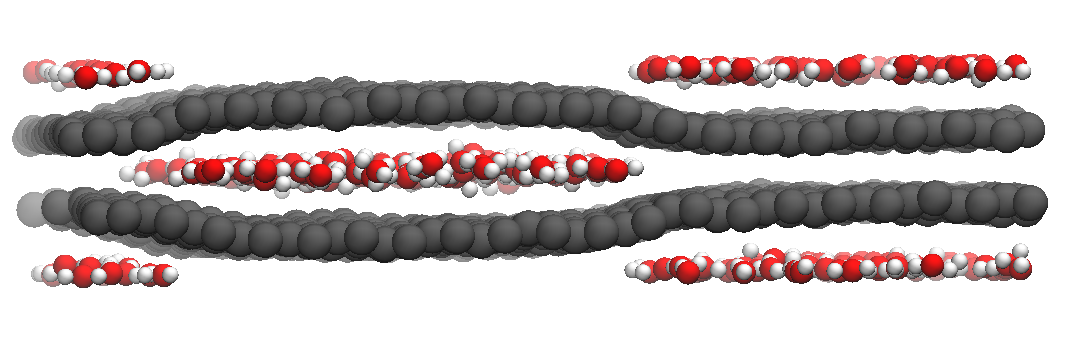
\includegraphics[width=0.99\linewidth]{d6L46_side} 
	(b)~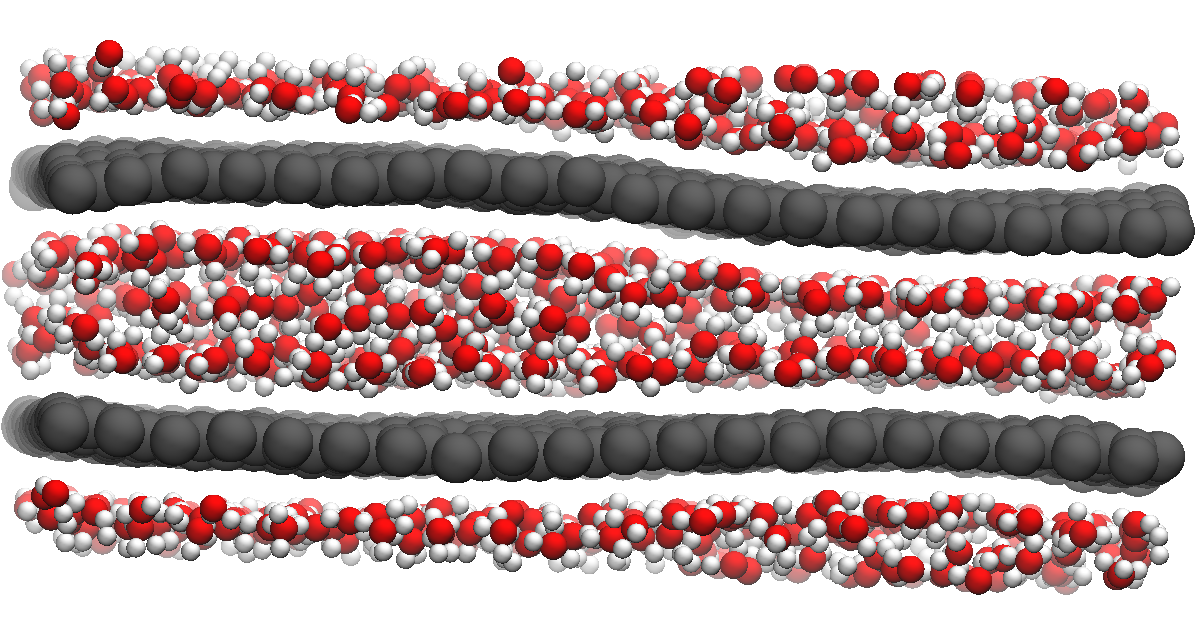
\includegraphics[width=0.95\linewidth]{d12L46_side}
	\vspace{-10pt}
	%\caption{ \textbf{\color{red} NEED PVarOX and PEI} \textit{Depictions of star polymer constituent chemistries.} (a) Adamantane core (b) Poly-delta-valerolactone monomer. (c) Poly-2,oxazoline with R-group pendant. The variations in R-group result in differing POX systems. For all POX, n = 24. } %, (d) Poly-ethylene glycol monomer, used as hydrophilic region for PVL variant systems. For all PEG blocks, n = 24.}
	\label{fig:chem_forms}
\end{figure}






\clearpage
\printbibliography
\end{document}












